%%
%% ----------------------------------------------------------------
%% Copyright (C) 2023-2024 by Simon Pfahler <simon.pfahler at ur dot de>
%% ----------------------------------------------------------------
%%
%! TeX program = lualatex
\DocumentMetadata{lang = en-us}
\documentclass{scrartcl}
\usepackage[left=4.5cm,right=3cm,top=3cm,bottom=3cm, marginpar=4cm]{geometry}
\setlength{\parindent}{0pt}
\setlength{\parskip}{1ex}

\usepackage{xcolor}
\usepackage{soul}

\usepackage{tikz}
\usetikzlibrary{positioning, shapes, fit, arrows.meta, decorations.pathmorphing, math}
\pgfdeclarelayer{bg}
\pgfsetlayers{bg,main}

\usepackage{pgfplots, pgfplotstable}
\pgfplotsset{compat=1.18}

%%%% from https://tex.stackexchange.com/questions/355713/pgfplots-show-error-marker-in-legend
\pgfplotsset{error bar legend/.style={%
    /pgfplots/legend image code/.prefix code={%
      \pgfkeysgetvalue{/pgfplots/error bars/error mark}{\pgfplotserrorbarsmark}%
      \draw[%
        /pgfplots/every error bar,
        mark=\pgfplotserrorbarsmark,
        /pgfplots/error bars/error mark options,
        sharp plot,
        ##1
      ] plot coordinates {(0.3cm, -0.15cm) (0.3cm, 0.15cm)};%
    }
  }
}
%%%%

\pgfplotsset{custom area legend/.style={%
    /pgfplots/legend image code/.prefix code={%
        \fill[##1, draw=white] plot coordinates {(0cm, -0.1cm) (0.6cm,-0.1cm) (0.6cm, 0.1cm) (0cm, 0.1cm)};%
    }
  }
}

\def\w{420pt}

\usepackage{hyperref}
\hypersetup{
    pdftitle={Easy colorblind-safe typesetting: the colorblind package},
    pdfauthor={Simon Pfahler},
}
\usepackage{cleveref}

\usepackage{csquotes}
\usepackage[backend=biber, style=numeric-comp, seconds=true, sorting=none, subentry=true, doi=false, alldates=iso]{biblatex}
\renewcommand*{\entrysetpunct}{\\[5pt]}
\addbibresource{bib.bib}

\usepackage[keep-defaults, Tol, OkabeIto, pgf]{colorblind}

\newcommand\colorblind{\textbf{colorblind} }
\newcommand\hlc[2][T-Q-PH4]{{%
    \colorlet{foo}{#1}%
    \sethlcolor{foo}\hl{#2}}%
}

\reversemarginpar
\newcommand\marg[1]{\leavevmode\marginpar{\raggedleft #1}}
\newcommand\tbs{\textbackslash}
\newcommand\cs[1]{\texttt{\tbs#1}}

\title{Easy colorblind-safe typesetting:\\ the \colorblind package}
\author{Simon Pfahler}
\date{\today\\Version 1.1}


\begin{document}

\maketitle

\begin{abstract}
	In colorblind-safe documents, the contents are presented in a way that the same information is conveyed to readers regardless of a potential color vision deficiency.
	This package provides some useful tools for colorblind-safe typesetting in \LaTeX.
	It provides color schemes for a wide range of applications.
	The most commonly used schemes are qualitative schemes, providing easily distinguishable colors for use in graphics, but also for text coloring or highlighting.
	Additionally, diverging and sequential schemes are provided, which can be used for encoding quantitative information using colors.
	This package incorporates colorblind-safeness into the writing process, making it both less cumbersome and less error-prone.
\end{abstract}

\tableofcontents
\clearpage

\section{Introduction}
\subsection{For the impatient}
Writing good colorblind-safe documents can be a tricky task.
It is a good starting point to realize that the default \LaTeX\ colors like \hlc[red]{red} or \hlc[blue]{blue} should be avoided.
This is why for the impatient, simply loading this package without specifying any options (i.e.\ \cs{usepackage\{colorblind\}}) redefines the default colors to more sensible alternatives.
\footnote{Where no suitable redefinition was possible for a builtin named color, the definition is changed to black.}

\begin{figure}[ht]
	\centering
	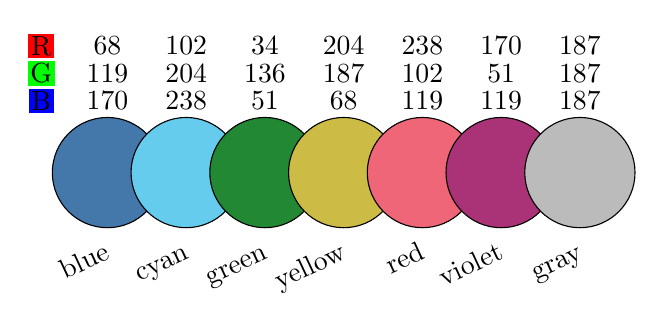
\begin{tikzpicture}
		\node[inner sep=1, fill=red] at (-1.2*0.7cm,2.3*0.7cm) {R};
		\node[inner sep=1, fill=green] at (-1.2*0.7cm, 1.8*0.7cm) {G};
		\node[inner sep=1, fill=blue] at (-1.2*0.7cm,1.3*0.7cm) {B};

		\node at (1*1cm-1cm,2.3*0.7cm) {68};
		\node at (1*1cm-1cm,1.8*0.7cm) {119};
		\node at (1*1cm-1cm,1.3*0.7cm) {170};
		\draw[fill=T-Q-B1] (1*1cm-1cm,0) circle (0.7cm);
		\node[rotate=25, anchor=north east] at (1*1cm-1cm,-1*0.7cm) {\vphantom{bp}blue};

		\node at (2*1cm-1cm,2.3*0.7cm) {102};
		\node at (2*1cm-1cm,1.8*0.7cm) {204};
		\node at (2*1cm-1cm,1.3*0.7cm) {238};
		\draw[fill=T-Q-B2] (2*1cm-1cm,0) circle (0.7cm);
		\node[rotate=25, anchor=north east] at (2*1cm-1cm,-1*0.7cm) {\vphantom{bp}cyan};

		\node at (3*1cm-1cm,2.3*0.7cm) {34};
		\node at (3*1cm-1cm,1.8*0.7cm) {136};
		\node at (3*1cm-1cm,1.3*0.7cm) {51};
		\draw[fill=T-Q-B3] (3*1cm-1cm,0) circle (0.7cm);
		\node[rotate=25, anchor=north east] at (3*1cm-1cm,-1*0.7cm) {\vphantom{bp}green};

		\node at (4*1cm-1cm,2.3*0.7cm) {204};
		\node at (4*1cm-1cm,1.8*0.7cm) {187};
		\node at (4*1cm-1cm,1.3*0.7cm) {68};
		\draw[fill=T-Q-B4] (4*1cm-1cm,0) circle (0.7cm);
		\node[rotate=25, anchor=north east] at (4*1cm-1cm,-1*0.7cm) {\vphantom{bp}yellow};

		\node at (5*1cm-1cm,2.3*0.7cm) {238};
		\node at (5*1cm-1cm,1.8*0.7cm) {102};
		\node at (5*1cm-1cm,1.3*0.7cm) {119};
		\draw[fill=T-Q-B5] (5*1cm-1cm,0) circle (0.7cm);
		\node[rotate=25, anchor=north east] at (5*1cm-1cm,-1*0.7cm) {\vphantom{bp}red};

		\node at (6*1cm-1cm,2.3*0.7cm) {170};
		\node at (6*1cm-1cm,1.8*0.7cm) {51};
		\node at (6*1cm-1cm,1.3*0.7cm) {119};
		\draw[fill=T-Q-B6] (6*1cm-1cm,0) circle (0.7cm);
		\node[rotate=25, anchor=north east] at (6*1cm-1cm,-1*0.7cm) {\vphantom{bp}violet};

		\node at (7*1cm-1cm,2.3*0.7cm) {187};
		\node at (7*1cm-1cm,1.8*0.7cm) {187};
		\node at (7*1cm-1cm,1.3*0.7cm) {187};
		\draw[fill=T-Q-B0] (7*1cm-1cm,0) circle (0.7cm);
		\node[rotate=25, anchor=north east] at (7*1cm-1cm,-1*0.7cm) {\vphantom{bp}gray};

	\end{tikzpicture}
	\caption{Redefinitions of the default \LaTeX\ colors.}
\end{figure}

It should be noted that this is a very brute-force way of trying to achieve colorblind-safeness.
If you care about this topic (which you should), the rest of this document provides details on how colorblind-safeness is best achieved in different scenarios.

\subsection{Package options}
\marg{\texttt{Tol}\\\texttt{OkabeIto}}%
The \colorblind package provides the color schemes by Paul Tol~\cite{Tol} and the Okabe Ito color palette~\cite{Ichihara_2008}.
By default, no schemes are loaded.
Providing one of the options \texttt{Tol} or \texttt{OkabeIto} loads all corresponding schemes.

\marg{\texttt{pgf}}%
If the option \texttt{pgf} is provided, continuous colormaps are defined for use with \texttt{pgfplots} (or \texttt{TikZ}).
Also, the command \cs{drawSchemeC} for drawing continuous color schemes is only defined when the option is provided and continuous color schemes are available (through providing the \texttt{Tol} option).
Continuous versions of color schemes are only available when the colors are allowed to be interpolated, see below for details.

\marg{\texttt{no-tikz}}%
The package uses \texttt{TikZ} to draw the discrete versions of color schemes.
Providing the option \texttt{no-tikz} disables this, the command \cs{drawScheme} is not defined in this case.

\marg{\texttt{keep-defaults}}%
The package redefines the default colors like \hlc[T-Q-PH5]{red} or \hlc[T-Q-PH1]{blue} to be colorblind-safe. By specifying this option, the defaults are not changed.

\subsection{Overview}
As an example for how to use the colors, we look at the \emph{bright qualitative} color scheme by Tol.
\cref{fig:T-Q-Bexample} shows the colors in the scheme.

\begin{figure}[ht]
	\centering
	\drawScheme{T-Q-B}
	\caption{Bright qualitative color scheme by Tol.}
	\label{fig:T-Q-Bexample}
\end{figure}

All colors in this model start with \texttt{T-Q-B}, indicating that it is a scheme by \textbf{T}ol, that it is a \textbf{q}ualitative scheme, and that it is the \textbf{b}right scheme.
The colors in the scheme are specified by a number following the scheme name, in this case ranging from \texttt{T-Q-B1} to \texttt{T-Q-B6} for the non-grey colors.
The additional color \texttt{T-Q-B0} provides a color that can be used, e.g., to indicate bad data.

There are two reasons why color names are not based on natural color names (e.g., ``\hlc[T-Q-PH1]{blue}''):
\begin{enumerate}
	\item Certain colors (\hlc[T-Q-PH3]{green}, \hlc[T-Q-PH5]{red}) are often used by people with full color vision to convey certain meanings (\hlc[T-Q-PH3]{good}, \hlc[T-Q-PH5]{bad}).
	      This meaning is difficult for people with color vision deficiencies to pick up.
	      By not using natural color names, it is easier to write colorblind-safe documents that do not make use of said connotations.
	\item Natural color names can be cumbersome, e.g., when slight variations of a color are used. It is annoying having to look up if a color is called, e.g., \hlc[T-Q-PH1]{blue} or \hlc[T-Q-PH2]{cyan}.
\end{enumerate}

These colors are used the same way as any other colors. To change the text color to \texttt{T-Q-B1} for example, use \cs{color\{T-Q-B1\}}.

\section{Guidelines}\label{sec:guidelines}
In this section, we provide some general guidelines for colorblind-safe design.

Color vision deficiencies apper in many different variations and grades of severity, up to monochromacy, where different colors can only be distinguished via their perceived brightness.
This means that while the color schemes provided by this package are easier to distinguish for the most common color vision deficiencies, information encoded only in color can never be truely colorblind safe.
This leads us to the most important rule in colorblind-safe design:
\begin{center}
	\setlength{\fboxrule}{1pt}
	\textbf{Rule 1}:
	\fbox{\parbox{0.65\columnwidth}{
			Always provide information in more ways than just color.
		}}
\end{center}

If this rule is satisfied in a document, it is by construction guaranteed to be colorblind-safe.
However, this does not mean that it is \emph{convenient} for people with color vision deficiencies to extract the information.
In order to achieve the best possible result, a few more rules should be considered when using color.
\begin{center}
	\setlength{\fboxrule}{1pt}
	\textbf{Rule 2}:
	\fbox{\parbox{0.65\columnwidth}{
			Stick to a color scheme.
			\begin{itemize}
				\item[(\textbf{a})] Do not mix colors within a scheme.
				\item[(\textbf{b})] Do not use shades of colors.
			\end{itemize}
		}}
\end{center}

Colors within colorblind-safe color schemes are designed to be eaily distinguishable for people with the most common color vision deficiencies, so we should only use colors from one color scheme in any given visual unit.
In extension, even colors from the same scheme should not be mixed, since this makes it harder to distinguish them.
Even if the result of the mixing is easily distinguishable for people with normal color vision, the same might not be true under certain color vision deficiencies.
For the same reaseon, shades of colors (i.e.\ mixings with black or white) should be avoided, because the brightness of colors is also used to make sure the colors are distinguishable.

\begin{center}
	\setlength{\fboxrule}{1pt}
	\textbf{Rule 3}:
	\fbox{\parbox{0.65\columnwidth}{
			Do not use color for information and aesthetics simultaneously.
		}}
\end{center}

Color is often also used for aesthetic reasons, e.g., on a scientific poster.
This is usually unproblematic, as the color does not convey information in this case.
However, if color is used to convey information in a visual unit, avoid using additional color for aesthetic purposes, as this makes it more difficult to extract the information encoded in the color.

\begin{center}
	\setlength{\fboxrule}{1pt}
	\textbf{Rule 4}:
	\fbox{\parbox{0.65\columnwidth}{
			Do not use rainbow color schemes.
		}}
\end{center}

Due to the many different colors in a rainbow color scheme, they are inevitably difficult to distinguish for people with color vision deficiencies.
Therefore, it is best to avoid them.
If a rainbow color scheme has to be used at all cost, Paul Tol (and thus also the \texttt{colorblind} package) provides both a discrete as well as a continuous version~\cite{Tol}, which are optimized to be as distinguishable as possible.

By following these four simple rules, we can ensure that the information encoded in a document is presented in a colorblind-safe way, and that it is reasonably convenient for people affected by color vision deficiencies to extract the information.
As a side node, following these rules leads to documents that do not suffer from information loss when printed in black and white, which is usually also desirable.

\section{Provided color schemes}\label{sec:colors}
The color schemes provided are split into three groups:
\begin{itemize}
	\item Qualitative schemes:\newline
	      These schemes are used to convey qualitative information, such as different data sources, countries or manufacturers.
	      They should usually be used for coloring text or distinguishing different lines/bars in a plot.
	\item Diverging color schemes:\newline
	      When quantitative data ranges between two extremes, and the middle is being considered ``neutral'', a diverging color scheme should be used.
	      Examples for this kind of data might be test grades, temperatures or pH values.
	\item Sequential color schemes:\newline
	      For quantitative data without an important midpoint, sequential color schemes should be preferred over diverging ones.
	      This is especially true for quantites that start from $0$.
	      They can be used to denote for example velocities, concentrations or pressures.
\end{itemize}

For each type of schemes, this package provides a range of options.
\Cref{sec:Tol_schemes} shows the schemes designed by Paul Tol~\cite{Tol}, which include qualitative, diverging and sequential schemes (see \cref{sec:T-Q,sec:T-D,sec:T-S}).
In \cref{sec:OkabeIto}, the Okabe Ito color scheme~\cite{Ichihara_2008} is provided, which is probably the most famous qualitative colorblind-safe color scheme due to it being mentioned in various articles in high-ranking journals.

All of the schemes are colorblind-safe, and some are optimized for printout or designed for a particular purpose.
This is denoted under the scheme name.\clearpage

\subsection{Paul Tol's color schemes}\label{sec:Tol_schemes}

\subsubsection{Qualitative color schemes}\label{sec:T-Q}
\begin{minipage}{0.5\textwidth}
	\centering
	\scalebox{0.7}{\drawScheme{T-Q-B}}\\
	\textbf{B}right\\
	\phantom{pb}
\end{minipage}\hfill%
\begin{minipage}{0.5\textwidth}
	\centering
	\scalebox{0.7}{\drawScheme{T-Q-V}}\\
	\textbf{V}ibrant
\end{minipage}

\begin{minipage}{0.5\textwidth}
	\centering
	\scalebox{0.7}{\drawScheme{T-Q-HC}}\\
	\textbf{H}igh-\textbf{C}ontrast\\
	works for black and white printout
\end{minipage}\hfill%
\begin{minipage}{0.5\textwidth}
	\centering
	\scalebox{0.7}{\drawScheme{T-Q-MC}}\\
	\textbf{M}edium-\textbf{C}ontrast\\
	works for black and white printout
\end{minipage}

\begin{center}
	\scalebox{0.7}{\drawScheme{T-Q-M}}\\
	\textbf{M}uted
\end{center}

\begin{minipage}{0.5\textwidth}
	\centering
	\scalebox{0.7}{\drawScheme{T-Q-PH}}\\
	\textbf{P}ale \textbf{H}ighlight\\
	specifically for text background
\end{minipage}\hfill%
\begin{minipage}{0.5\textwidth}
	\centering
	\scalebox{0.7}{\drawScheme{T-Q-DT}}\\
	\textbf{D}ark \textbf{T}ext\\
	specifically for text color
\end{minipage}

\begin{center}
	\scalebox{0.7}{\drawScheme{T-Q-L}}\\
	\textbf{L}ight\\
	less distinguishable than other schemes,\\ mostly meant for filling in labelled cells
\end{center}\clearpage

\subsubsection{Diverging color schemes}\label{sec:T-D}
For diverging schemes, when a continuous scheme is needed, the colors are allowed to be linearly interpolated.
When using the option \texttt{pgf}, the interpolations are available as colormaps with the names of their color scheme.

\begin{center}
	\scalebox{0.7}{\drawScheme{T-D-S}}\\
	\drawSchemeC[0.6\textwidth]{T-D-S}\\
	\textbf{S}unset
\end{center}

\begin{center}
	\scalebox{0.7}{\drawScheme{T-D-N}}\\
	\drawSchemeC[0.9\textwidth]{T-D-N}\\
	\textbf{N}ightfall
\end{center}

\begin{center}
	\scalebox{0.7}{\drawScheme{T-D-BR}}\\
	\drawSchemeC[0.5\textwidth]{T-D-BR}\\
	\textbf{B}u\textbf{R}d
\end{center}

\begin{center}
	\scalebox{0.7}{\drawScheme{T-D-PG}}\\
	\drawSchemeC[0.5\textwidth]{T-D-PG}\\
	\textbf{P}R\textbf{G}n
\end{center}\clearpage

\subsubsection{Sequential color schemes}\label{sec:T-S}
For most sequential schemes, a continuous scheme can be obtained again by linearly interpolating the colors.
The only exception to this is the \emph{discrete rainbow} scheme, which has an explicitly continuos variation, the \emph{smooth rainbow} scheme.
When using the option \texttt{pgf}, the interpolations are available as colormaps with the names of their color scheme.

When the discrete scheme is not shown, this is because there are too many colors in it.

\begin{center}
	\scalebox{0.7}{\drawScheme{T-S-YOB}}\\
	\drawSchemeC[0.5\textwidth]{T-S-YOB}\\
	\textbf{Y}l\textbf{O}r\textbf{B}r
\end{center}

\begin{center}
	\drawSchemeC[0.9\textwidth]{T-S-IR}\\
	\textbf{Ir}idescent
\end{center}

\begin{center}
	\scalebox{0.7}{\drawScheme{T-S-IN}}\\
	\drawSchemeC[0.6\textwidth]{T-S-IN}\\
	\textbf{In}candescent\\
	not print-friendly
\end{center}

\begin{center}
	\scalebox{0.7}{\drawScheme{T-S-DR}}\\
	\textbf{D}iscrete \textbf{R}ainbow\\
	Do not interpolate!
\end{center}

\begin{center}
	\drawSchemeC[\textwidth]{T-S-SR}\\
	\textbf{S}mooth \textbf{R}ainbow\\
\end{center}\clearpage

\subsection{Okabe Ito qualitative color scheme}\label{sec:OkabeIto}
This is the qualitative color scheme commonly known as the \emph{Okabe Ito} color palette~\cite{Ichihara_2008}.

\begin{center}
	\scalebox{0.7}{\drawScheme{OI}}\\
	\textbf{O}kabe \textbf{I}to
\end{center}

\section{Notes on color models}
To digitally represent a color, we need to choose a color model, e.g.\ \texttt{rgb} or \texttt{cmyk}.
The colors provided by this package were originally defined in RGB-based color models like \texttt{rgb} or \texttt{html}.
Therefore, \texttt{RGB} definitions are used when no color model is specified explicitly.
In the vast majority of use cases, no such color model should be specified.
The reason for this is that modern devices like printers and screens have their own built-in conversion tables between color models, which provide better conversion than some generic formula can.
For example when sending a document to a printer, all colors (even colors already specified in \texttt{cymk}) are converted to this device's specific \texttt{cmyk} color model and ink is put on the paper according to these device-specific numbers.
Manually converting \texttt{rgb} to \texttt{cmyk} beforehand is therefore not beneficial, as a conversion always has to be performed anyways.

Due to technical reasons in very rare use-cases, definitions in \texttt{cmyk} are necessary and are also provided.
It is strongly discouraged that you use the \texttt{cmyk} color model, unless you have a very good reason why you need it.
The only good reason I came across so far is that you send your document to someone else for printing and that person refuses to print your document unless you specify your colors in the \texttt{cmyk} color model\footnote{This may sound unreasonable, but precisely this happened with the printing house of a very well-known \LaTeX\ book.}.
In particular and as mentioned above, \texttt{cmyk} should not be used just because you want to print a document.
Let the printer handle conversion in that case.

\section{Provided commands}
\marg{\cs{drawScheme\{...\}}}%
The discrete visualizations of color schemes given in this documentation are created with the command \cs{drawScheme\{...\}}.
The name of the color scheme should be provided to the command, e.g.\ \cs{drawScheme\{T-Q-B\}} to print the \emph{qualitative bright} scheme by Tol.
Note that this command is not available when the package option \texttt{no-tikz} is used.

\marg{\cs{drawSchemeC\{...\}}}%
The continuous visualizations of color schemes given in this documentation are created with the command \cs{drawSchemeC\{...\}}.
The name of the color scheme should be provided to the command, e.g.\ \cs{drawSchemeC\{T-D-S\}} to print the \emph{diverging sunset} scheme by Tol.
Note that this command only works for color schemes that are allowed to be interpolated, and that the command is only available when the package option \texttt{pgf} is used.

\clearpage
\printbibliography

\end{document}
